\documentclass[ignorenonframetext,]{beamer}
\setbeamertemplate{caption}[numbered]
\setbeamertemplate{caption label separator}{: }
\setbeamercolor{caption name}{fg=normal text.fg}
\beamertemplatenavigationsymbolsempty
\usepackage{lmodern}
\usepackage{amssymb,amsmath}
\usepackage{ifxetex,ifluatex}
\usepackage{fixltx2e} % provides \textsubscript
\ifnum 0\ifxetex 1\fi\ifluatex 1\fi=0 % if pdftex
\usepackage[T1]{fontenc}
\usepackage[utf8]{inputenc}
\else % if luatex or xelatex
\ifxetex
\usepackage{mathspec}
\else
\usepackage{fontspec}
\fi
\defaultfontfeatures{Ligatures=TeX,Scale=MatchLowercase}
\fi
% use upquote if available, for straight quotes in verbatim environments
\IfFileExists{upquote.sty}{\usepackage{upquote}}{}
% use microtype if available
\IfFileExists{microtype.sty}{%
\usepackage{microtype}
\UseMicrotypeSet[protrusion]{basicmath} % disable protrusion for tt fonts
}{}
\newif\ifbibliography
\usepackage{color}
\usepackage{fancyvrb}
\newcommand{\VerbBar}{|}
\newcommand{\VERB}{\Verb[commandchars=\\\{\}]}
\DefineVerbatimEnvironment{Highlighting}{Verbatim}{commandchars=\\\{\}}
% Add ',fontsize=\small' for more characters per line
\usepackage{framed}
\definecolor{shadecolor}{RGB}{248,248,248}
\newenvironment{Shaded}{\begin{snugshade}}{\end{snugshade}}
\newcommand{\KeywordTok}[1]{\textcolor[rgb]{0.13,0.29,0.53}{\textbf{{#1}}}}
\newcommand{\DataTypeTok}[1]{\textcolor[rgb]{0.13,0.29,0.53}{{#1}}}
\newcommand{\DecValTok}[1]{\textcolor[rgb]{0.00,0.00,0.81}{{#1}}}
\newcommand{\BaseNTok}[1]{\textcolor[rgb]{0.00,0.00,0.81}{{#1}}}
\newcommand{\FloatTok}[1]{\textcolor[rgb]{0.00,0.00,0.81}{{#1}}}
\newcommand{\ConstantTok}[1]{\textcolor[rgb]{0.00,0.00,0.00}{{#1}}}
\newcommand{\CharTok}[1]{\textcolor[rgb]{0.31,0.60,0.02}{{#1}}}
\newcommand{\SpecialCharTok}[1]{\textcolor[rgb]{0.00,0.00,0.00}{{#1}}}
\newcommand{\StringTok}[1]{\textcolor[rgb]{0.31,0.60,0.02}{{#1}}}
\newcommand{\VerbatimStringTok}[1]{\textcolor[rgb]{0.31,0.60,0.02}{{#1}}}
\newcommand{\SpecialStringTok}[1]{\textcolor[rgb]{0.31,0.60,0.02}{{#1}}}
\newcommand{\ImportTok}[1]{{#1}}
\newcommand{\CommentTok}[1]{\textcolor[rgb]{0.56,0.35,0.01}{\textit{{#1}}}}
\newcommand{\DocumentationTok}[1]{\textcolor[rgb]{0.56,0.35,0.01}{\textbf{\textit{{#1}}}}}
\newcommand{\AnnotationTok}[1]{\textcolor[rgb]{0.56,0.35,0.01}{\textbf{\textit{{#1}}}}}
\newcommand{\CommentVarTok}[1]{\textcolor[rgb]{0.56,0.35,0.01}{\textbf{\textit{{#1}}}}}
\newcommand{\OtherTok}[1]{\textcolor[rgb]{0.56,0.35,0.01}{{#1}}}
\newcommand{\FunctionTok}[1]{\textcolor[rgb]{0.00,0.00,0.00}{{#1}}}
\newcommand{\VariableTok}[1]{\textcolor[rgb]{0.00,0.00,0.00}{{#1}}}
\newcommand{\ControlFlowTok}[1]{\textcolor[rgb]{0.13,0.29,0.53}{\textbf{{#1}}}}
\newcommand{\OperatorTok}[1]{\textcolor[rgb]{0.81,0.36,0.00}{\textbf{{#1}}}}
\newcommand{\BuiltInTok}[1]{{#1}}
\newcommand{\ExtensionTok}[1]{{#1}}
\newcommand{\PreprocessorTok}[1]{\textcolor[rgb]{0.56,0.35,0.01}{\textit{{#1}}}}
\newcommand{\AttributeTok}[1]{\textcolor[rgb]{0.77,0.63,0.00}{{#1}}}
\newcommand{\RegionMarkerTok}[1]{{#1}}
\newcommand{\InformationTok}[1]{\textcolor[rgb]{0.56,0.35,0.01}{\textbf{\textit{{#1}}}}}
\newcommand{\WarningTok}[1]{\textcolor[rgb]{0.56,0.35,0.01}{\textbf{\textit{{#1}}}}}
\newcommand{\AlertTok}[1]{\textcolor[rgb]{0.94,0.16,0.16}{{#1}}}
\newcommand{\ErrorTok}[1]{\textcolor[rgb]{0.64,0.00,0.00}{\textbf{{#1}}}}
\newcommand{\NormalTok}[1]{{#1}}
\usepackage{longtable,booktabs}
\usepackage{caption}
% These lines are needed to make table captions work with longtable:
\makeatletter
\def\fnum@table{\tablename~\thetable}
\makeatother
\usepackage{graphicx,grffile}
\makeatletter
\def\maxwidth{\ifdim\Gin@nat@width>\linewidth\linewidth\else\Gin@nat@width\fi}
\def\maxheight{\ifdim\Gin@nat@height>\textheight0.8\textheight\else\Gin@nat@height\fi}
\makeatother
% Scale images if necessary, so that they will not overflow the page
% margins by default, and it is still possible to overwrite the defaults
% using explicit options in \includegraphics[width, height, ...]{}
\setkeys{Gin}{width=\maxwidth,height=\maxheight,keepaspectratio}

% Prevent slide breaks in the middle of a paragraph:
\widowpenalties 1 10000
\raggedbottom

\AtBeginPart{
\let\insertpartnumber\relax
\let\partname\relax
\frame{\partpage}
}
\AtBeginSection{
\ifbibliography
\else
\let\insertsectionnumber\relax
\let\sectionname\relax
\frame{\sectionpage}
\fi
}
\AtBeginSubsection{
\let\insertsubsectionnumber\relax
\let\subsectionname\relax
\frame{\subsectionpage}
}

\setlength{\parindent}{0pt}
\setlength{\parskip}{6pt plus 2pt minus 1pt}
\setlength{\emergencystretch}{3em}  % prevent overfull lines
\providecommand{\tightlist}{%
\setlength{\itemsep}{0pt}\setlength{\parskip}{0pt}}
\setcounter{secnumdepth}{0}
% declare overall beamer theme to use as baseline
%\usetheme{default}

% make code-output smaller
\DefineVerbatimEnvironment{Highlighting}{Verbatim}{fontsize=\tiny,commandchars=\\\{\}}

% make console-output smaller:
  \makeatletter
\def\verbatim{\tiny\@verbatim \frenchspacing\@vobeyspaces \@xverbatim}
\makeatother


\setlength{\parskip}{0pt}


\setlength{\OuterFrameSep}{-4pt}
\makeatletter
\preto{\@verbatim}{\topsep=-10pt \partopsep=-10pt }
\makeatother

\title{Hogyan modellezzük betegségek előfordulásának időbeli változását?}
\author{Ferenci Tamás\(^1\) \and Kolossváry Endre\(^2\)}
\institute{\(^1\)Óbudai Egyetem, Neumann János Informatikai Kar, Élettani
Szabályozások Kutatóközpont \and \(^2\)Szent Imre Egyetemi Oktatókórház, Angiológiai Osztály}
\date{2017. június 9.}

\begin{document}
\frame{\titlepage}

\begin{frame}
\tableofcontents[hideallsubsections]
\end{frame}

\section{Bevezetés, klasszikus
megoldások}\label{bevezetes-klasszikus-megoldasok}

\begin{frame}{Betegségek előfordulásának időbeli változása}

\begin{itemize}
\tightlist
\item
  Az epidemiológiai egyik alapvető kérdése
\item
  Számos előfordulási adat érhető el idősorosan
\item
  Könnyen gyártható is ilyen adminisztratív/finanszírozási adatokból
\item
  Klasszikus elemzési eszköztár (különböző időtartamokra aggregálás és
  ábrázolás, standardizálás stb.) vs.~korszerű -- regressziós --
  modellezés
\end{itemize}

\end{frame}

\begin{frame}{A regressziós modellezés előnyei és hátrányai}

Előnyök:

\begin{itemize}
\tightlist
\item
  Több tényező figyelembevétele teljesen kézenfekvő
\item
  ,,Beépített'' standardizálás
\item
  Jól felhasználható (interpretálható, ábrázolható, CI-vel ellátható
  stb.) eredmények
\item
  Kiforrott apparátus, jó számítástechnikai támogatás
\end{itemize}

Hátrányok:

\begin{itemize}
\tightlist
\item
  A modellfeltevések maguk is bejönnek, teljesülésük kérdés, ellenőrizni
  kell őket
\end{itemize}

\end{frame}

\begin{frame}{Esettanulmány}

\begin{itemize}
\tightlist
\item
  Alsó végtagi érbetegségek talaján előforduló major amputációk
\item
  Adatforrás: ÁEEK (adminisztratív/finanszírozási adatbázis)
\item
  2004-től 2014-ig tart a most vizsgált idősor
\item
  Ismert az alany neme és életkora (számos más is, de azokat most nem
  használjuk)
\end{itemize}

\end{frame}

\begin{frame}{Függvényforma-választás}

Klasszikusan: paraméteres (pl. \(\beta_0+\beta_{Year} Year\))
vs.~nem-paraméteres (pl.
\(\beta_0+\beta_{Year=2005}D_{Year=2005}+\beta_{Year=2006}D_{Year=2006}+\ldots+\beta_{Year=2014}D_{Year=2014}\))

\end{frame}

\begin{frame}[fragile]{Nemparaméteres függvényforma (az év példáján)}

\begin{Shaded}
\begin{Highlighting}[]
\NormalTok{fit.nempara <-}\StringTok{ }\KeywordTok{Glm}\NormalTok{( N ~}\StringTok{ }\KeywordTok{scored}\NormalTok{( Year ) +}\StringTok{ }\KeywordTok{scored}\NormalTok{( Month ) +}\StringTok{ }\NormalTok{SEX*}\KeywordTok{rcs}\NormalTok{( AgeCut ),}
                    \DataTypeTok{offset =} \KeywordTok{log}\NormalTok{( Population ), }\DataTypeTok{data =} \NormalTok{TimeStratified,}
                    \DataTypeTok{family =} \KeywordTok{poisson}\NormalTok{( }\DataTypeTok{link =} \NormalTok{log ) )}
\KeywordTok{plot}\NormalTok{( }\KeywordTok{Predict}\NormalTok{( fit.nempara, }\DataTypeTok{fun =} \NormalTok{exp100k, Year, }\DataTypeTok{Month =} \DecValTok{6} \NormalTok{), }\DataTypeTok{ylim =} \KeywordTok{c}\NormalTok{( }\DecValTok{18}\NormalTok{, }\DecValTok{25} \NormalTok{) )}
\end{Highlighting}
\end{Shaded}

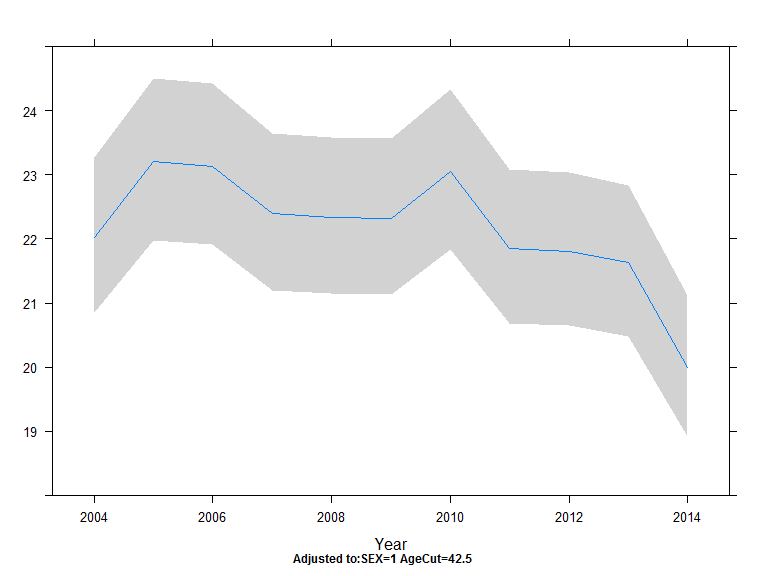
\includegraphics{BiometriaiKonf2017_FerenciKolossvary_files/figure-beamer/nemparameteres-1.pdf}

\end{frame}

\begin{frame}[fragile]{Paraméteres függvényforma (az év példáján)}

\begin{Shaded}
\begin{Highlighting}[]
\NormalTok{fit.para <-}\StringTok{ }\KeywordTok{Glm}\NormalTok{( N ~}\StringTok{ }\NormalTok{Year +}\StringTok{ }\KeywordTok{scored}\NormalTok{( Month ) +}\StringTok{ }\NormalTok{SEX*}\KeywordTok{rcs}\NormalTok{( AgeCut ),}
                 \DataTypeTok{offset =} \KeywordTok{log}\NormalTok{( Population ), }\DataTypeTok{data =} \NormalTok{TimeStratified,}
                 \DataTypeTok{family =} \KeywordTok{poisson}\NormalTok{( }\DataTypeTok{link =} \NormalTok{log ) )}
\KeywordTok{plot}\NormalTok{( }\KeywordTok{Predict}\NormalTok{( fit.para, }\DataTypeTok{fun =} \NormalTok{exp100k, Year, }\DataTypeTok{Month =} \DecValTok{6} \NormalTok{), }\DataTypeTok{ylim =} \KeywordTok{c}\NormalTok{( }\DecValTok{18}\NormalTok{, }\DecValTok{25} \NormalTok{) )}
\end{Highlighting}
\end{Shaded}

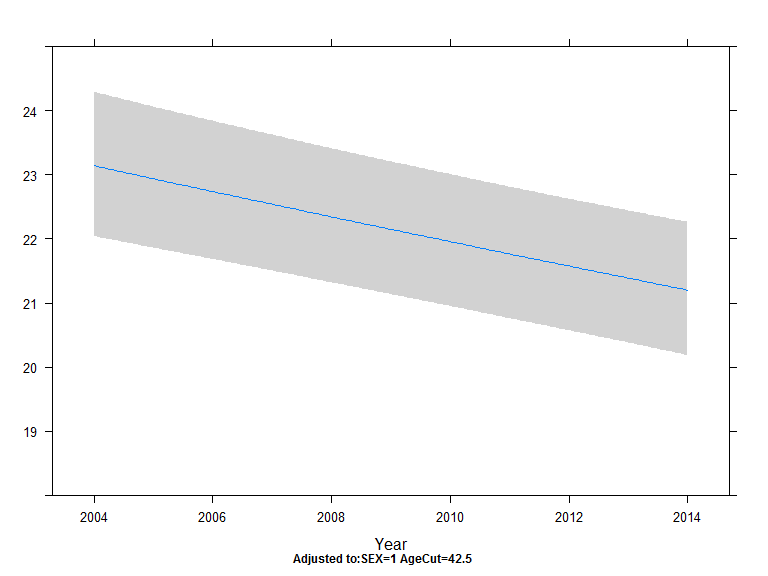
\includegraphics{BiometriaiKonf2017_FerenciKolossvary_files/figure-beamer/parameteres-1.pdf}

\end{frame}

\begin{frame}{Nemparaméteres vs.~paraméteres: szempontok a választáshoz}

\begin{itemize}
\tightlist
\item
  Illeszkedés jósága vs.~takarékosság (és ebből adódóan: becsülhetőség,
  általánosítóképesség)
\end{itemize}

\begin{longtable}[]{@{}lrrr@{}}
\toprule
Függvényforma & df & \(\chi^2\) & AIC\tabularnewline
\midrule
\endhead
Nemparaméteres & 31 & 102725.1 & 16160.11\tabularnewline
Paraméteres & 22 & 102686.2 & 16181.01\tabularnewline
\bottomrule
\end{longtable}

\begin{itemize}
\tightlist
\item
  Klinikai interpretálhatóság
\item
  Időbeli extrapolálhatóság
\end{itemize}

\end{frame}

\section{Egy fél-paraméteres megoldás: spline-ok
használata}\label{egy-fel-parameteres-megoldas-spline-ok-hasznalata}

\begin{frame}[allowframebreaks]{A spline-ok lényege}

\begin{itemize}
\tightlist
\item
  Technikailag paraméteres, de olyan komplex a függvényforma, hogy
  úgysem interpretáljuk
\item
  Alapgondolat: cserében ezért kapjunk olyan megoldást, ami egyszerre
  flexibilis (mint a nem-paraméteresek), de közben takarékos a
  szabadsági fokokkal (mint a paraméteresek)
\item
  Egymondatos definíció: a spline szakaszonként definiált polinomokból
  összerakott görbe (úgy, hogy a szakaszok találkozási pontjánál, a
  csomópontoknál szép simán menjenek át egymásba)
\item
  Talán a leggyakoribb a korlátozott köbös spline: harmadfokú polinomok,
  a csomópontoknál azonos érték, derivált és második derivált
  (belátható, hogy ez azt fogja jelenteni, hogy egy globális harmadfokú
  függvényt kell venni, és szakaszonként csak a harmadfokú tagot kell
  eltéríteni), az első pont előtt és az utolsó után pedig lineárisan
  megy tovább (ez még tovább egyszerűsít)
\item
  \(k\) csomópont esetén \(k-1\) paramétert kell becsülni (a csomópontok
  számát és helyét általában nem statisztikai becsléssel határozzuk meg)
\end{itemize}

\end{frame}

\begin{frame}[fragile]{Emlékeztetőül: nemparaméteres függfényvforma}

\begin{Shaded}
\begin{Highlighting}[]
\NormalTok{fit.nempara <-}\StringTok{ }\KeywordTok{Glm}\NormalTok{( N ~}\StringTok{ }\KeywordTok{scored}\NormalTok{( Year ) +}\StringTok{ }\KeywordTok{scored}\NormalTok{( Month ) +}\StringTok{ }\NormalTok{SEX*}\KeywordTok{rcs}\NormalTok{( AgeCut ),}
                    \DataTypeTok{offset =} \KeywordTok{log}\NormalTok{( Population ), }\DataTypeTok{data =} \NormalTok{TimeStratified,}
                    \DataTypeTok{family =} \KeywordTok{poisson}\NormalTok{( }\DataTypeTok{link =} \NormalTok{log ) )}
\KeywordTok{plot}\NormalTok{( }\KeywordTok{Predict}\NormalTok{( fit.nempara, }\DataTypeTok{fun =} \NormalTok{exp100k, Year, }\DataTypeTok{Month =} \DecValTok{6} \NormalTok{), }\DataTypeTok{ylim =} \KeywordTok{c}\NormalTok{( }\DecValTok{18}\NormalTok{, }\DecValTok{25} \NormalTok{) )}
\end{Highlighting}
\end{Shaded}

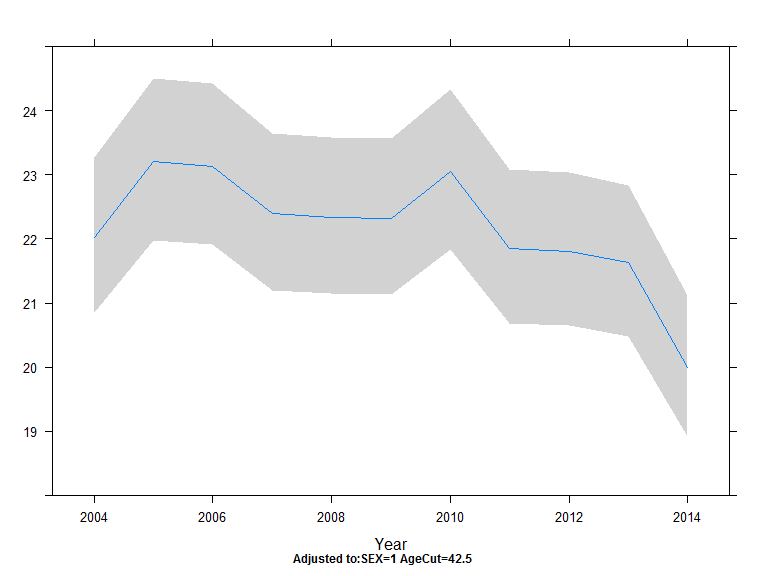
\includegraphics{BiometriaiKonf2017_FerenciKolossvary_files/figure-beamer/nemparameteres2-1.pdf}

\end{frame}

\begin{frame}[fragile]{Emlékeztetőül: paraméteres függfényvforma}

\begin{Shaded}
\begin{Highlighting}[]
\NormalTok{fit.para <-}\StringTok{ }\KeywordTok{Glm}\NormalTok{( N ~}\StringTok{ }\NormalTok{Year +}\StringTok{ }\KeywordTok{scored}\NormalTok{( Month ) +}\StringTok{ }\NormalTok{SEX*}\KeywordTok{rcs}\NormalTok{( AgeCut ),}
                 \DataTypeTok{offset =} \KeywordTok{log}\NormalTok{( Population ), }\DataTypeTok{data =} \NormalTok{TimeStratified,}
                 \DataTypeTok{family =} \KeywordTok{poisson}\NormalTok{( }\DataTypeTok{link =} \NormalTok{log ) )}
\KeywordTok{plot}\NormalTok{( }\KeywordTok{Predict}\NormalTok{( fit.para, }\DataTypeTok{fun =} \NormalTok{exp100k, Year, }\DataTypeTok{Month =} \DecValTok{6} \NormalTok{), }\DataTypeTok{ylim =} \KeywordTok{c}\NormalTok{( }\DecValTok{18}\NormalTok{, }\DecValTok{25} \NormalTok{) )}
\end{Highlighting}
\end{Shaded}

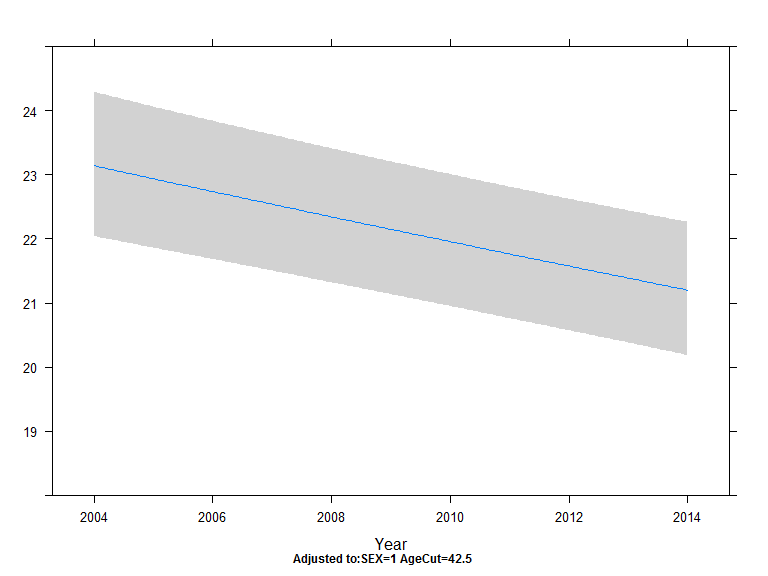
\includegraphics{BiometriaiKonf2017_FerenciKolossvary_files/figure-beamer/parameteres2-1.pdf}

\end{frame}

\begin{frame}[fragile]{És a spline-okkal történő megoldás}

\begin{Shaded}
\begin{Highlighting}[]
\NormalTok{fit.spline <-}\StringTok{ }\KeywordTok{Glm}\NormalTok{( N ~}\StringTok{ }\KeywordTok{rcs}\NormalTok{( Year ) +}\StringTok{ }\KeywordTok{scored}\NormalTok{( Month ) +}\StringTok{ }\NormalTok{SEX*}\KeywordTok{rcs}\NormalTok{( AgeCut ),}
                   \DataTypeTok{offset =} \KeywordTok{log}\NormalTok{( Population ), }\DataTypeTok{data =} \NormalTok{TimeStratified,}
                   \DataTypeTok{family =} \KeywordTok{poisson}\NormalTok{( }\DataTypeTok{link =} \NormalTok{log ) )}
\KeywordTok{plot}\NormalTok{( }\KeywordTok{Predict}\NormalTok{( fit.spline, }\DataTypeTok{fun =} \NormalTok{exp100k, Year, }\DataTypeTok{Month =} \DecValTok{6} \NormalTok{), }\DataTypeTok{ylim =} \KeywordTok{c}\NormalTok{( }\DecValTok{18}\NormalTok{, }\DecValTok{25} \NormalTok{) )}
\end{Highlighting}
\end{Shaded}

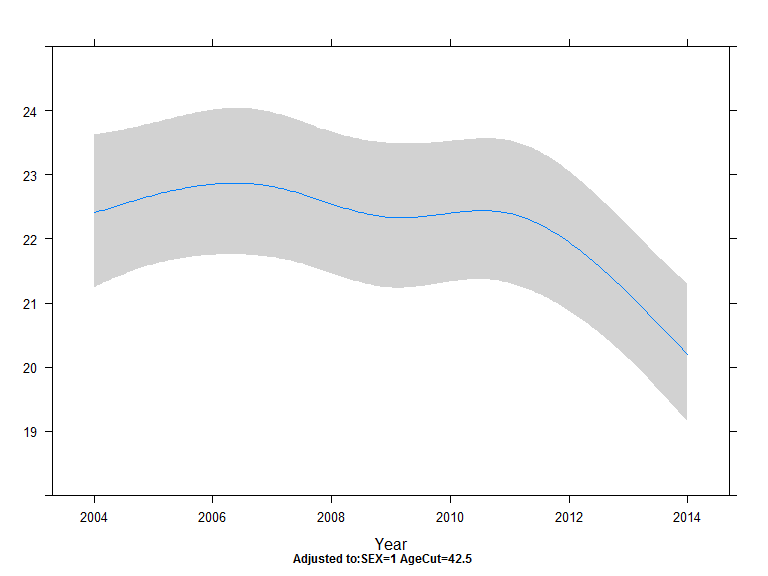
\includegraphics{BiometriaiKonf2017_FerenciKolossvary_files/figure-beamer/spline-1.pdf}

\end{frame}

\begin{frame}{Összehasonlítás}

\begin{itemize}
\tightlist
\item
  Illeszkedés jósága vs.~takarékosság
\end{itemize}

\begin{longtable}[]{@{}lrrr@{}}
\toprule
Függvényforma & df & \(\chi^2\) & AIC\tabularnewline
\midrule
\endhead
Nemparaméteres & 31 & 102725.1 & 16160.11\tabularnewline
Spline & 25 & 102709.8 & 16163.42\tabularnewline
Paraméteres & 22 & 102686.2 & 16181.01\tabularnewline
\bottomrule
\end{longtable}

\begin{itemize}
\tightlist
\item
  Klinikai interpretálhatóság
\item
  Időbeli extrapolálhatóság
\end{itemize}

\end{frame}

\section{Interpretálhatóság javítása a félparaméteres
megoldásnál}\label{interpretalhatosag-javitasa-a-felparameteres-megoldasnal}

\begin{frame}{Az alapgondolat}

\begin{itemize}
\tightlist
\item
  Mi érdekel minket elsősorban?
\item
  Az egyik nagyon fontos kérdés: mikor vált ritkábbá (vagy épp
  gyakoribbá) a betegség?
\item
  Lefordítva: a függvényforma deriváltját keressük!
\end{itemize}

\end{frame}

\begin{frame}{Véges differenciák módszere}

\begin{itemize}
\tightlist
\item
  A paraméteres függvényformák triviális deriválhatóak (pláne a
  lineáris), de mi a helyzet a spline-okkal?
\item
  Elég nyakatekert, de szerencsére egy huszárvágással megoldhatjuk az
  egész problémát
\item
  A deriválást közelítve \emph{bármilyen} függvényformára meg tudjuk
  oldani a problémát; kissé nagyképűen szólva, a véges differenciák
  módszerét alkalmazzuk: \[
  f'\left(x\right)=\frac{f\left(x+h\right)-f\left(x\right)}{h}\Bigg\rvert_{h \textrm{ kicsi}}
  \]
\end{itemize}

\end{frame}

\begin{frame}[fragile]{Spline deriválás véges differenciák módszerével
R-ben}

Szerencsére Gavin Simpson már eleve megírta nekünk az \texttt{mgcv}
csomaghoz illeszkedően:

\begin{itemize}
\tightlist
\item
  Github:
  \href{https://gist.github.com/gavinsimpson/e73f011fdaaab4bb5a30}{gavinsimpson
  / Deriv.R}
\item
  Github:
  \href{https://gist.github.com/gavinsimpson/ca18c9c789ef5237dbc6}{gavinsimpson
  / derivSimulCI.R}
\end{itemize}

A releváns kódrészlet:

\begin{Shaded}
\begin{Highlighting}[]
\NormalTok{X0 <-}\StringTok{ }\KeywordTok{predict}\NormalTok{(mod, newDF, }\DataTypeTok{type =} \StringTok{"lpmatrix"}\NormalTok{)}
\NormalTok{newDF <-}\StringTok{ }\NormalTok{newDF +}\StringTok{ }\NormalTok{eps}
\NormalTok{X1 <-}\StringTok{ }\KeywordTok{predict}\NormalTok{(mod, newDF, }\DataTypeTok{type =} \StringTok{"lpmatrix"}\NormalTok{)}
\NormalTok{Xp <-}\StringTok{ }\NormalTok{(X1 -}\StringTok{ }\NormalTok{X0) /}\StringTok{ }\NormalTok{eps}
\end{Highlighting}
\end{Shaded}

\end{frame}

\begin{frame}[fragile]{Az eredmény}

\begin{Shaded}
\begin{Highlighting}[]
\NormalTok{fit <-}\StringTok{ }\KeywordTok{gam}\NormalTok{( N ~}\StringTok{ }\KeywordTok{s}\NormalTok{( Year ) +}\StringTok{ }\KeywordTok{s}\NormalTok{( Month, }\DataTypeTok{bs =} \StringTok{"cc"} \NormalTok{) +}\StringTok{ }\KeywordTok{s}\NormalTok{( AgeCut, }\DataTypeTok{by =} \NormalTok{SEX ) +}\StringTok{ }\NormalTok{SEX,}
            \DataTypeTok{offset =} \KeywordTok{log}\NormalTok{( Population ), }\DataTypeTok{data =} \NormalTok{TimeStratified, }\DataTypeTok{family =} \StringTok{"poisson"} \NormalTok{)}
\NormalTok{fit.d <-}\StringTok{ }\KeywordTok{Deriv}\NormalTok{( fit, }\DataTypeTok{n =} \DecValTok{1000}\NormalTok{, }\DataTypeTok{m.terms.var =} \KeywordTok{c}\NormalTok{( }\StringTok{"Year"}\NormalTok{, }\StringTok{"Month"}\NormalTok{, }\StringTok{"AgeCut"} \NormalTok{),}
                \DataTypeTok{newdatafix =} \KeywordTok{data.frame}\NormalTok{( }\DataTypeTok{SEX =} \KeywordTok{as.factor}\NormalTok{( }\DecValTok{1} \NormalTok{) ) )}
\KeywordTok{plot}\NormalTok{( fit.d, }\DataTypeTok{term =} \StringTok{"Year"}\NormalTok{, }\DataTypeTok{alpha =} \DecValTok{1} \NormalTok{)}
\end{Highlighting}
\end{Shaded}

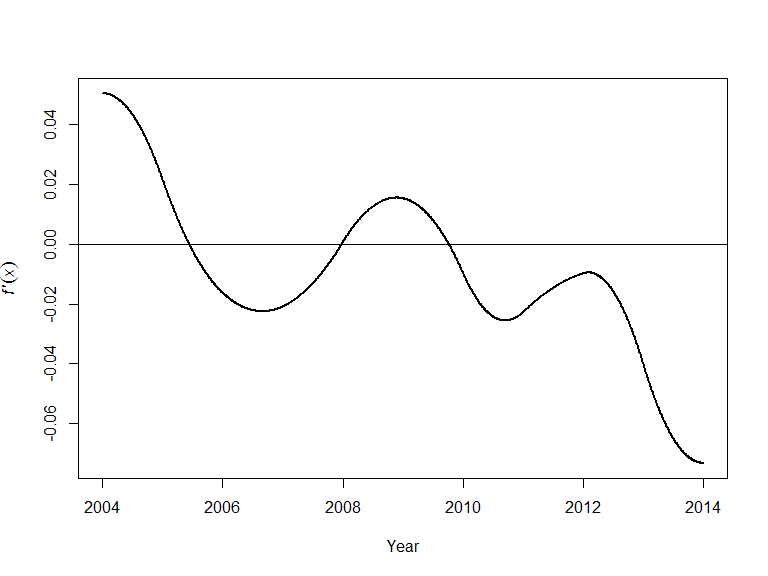
\includegraphics{BiometriaiKonf2017_FerenciKolossvary_files/figure-beamer/splinederivkod-1.pdf}

\end{frame}

\begin{frame}[fragile]{De a poén csak most jön}

\begin{itemize}
\tightlist
\item
  A deriválás azért nem volt egy akkor tudományos eredmény\dots{}
\item
  Jó lenne tudni azt is, hogy ez hol szignifikáns!
\item
  Most jön a szép rész: a deriváltra tudunk konfidenciaintervallumot is
  adni!
\end{itemize}

\begin{Shaded}
\begin{Highlighting}[]
\NormalTok{for(i in }\KeywordTok{seq_len}\NormalTok{(nt)) \{}
  \NormalTok{Xi <-}\StringTok{ }\NormalTok{Xp *}\StringTok{ }\DecValTok{0}
  \NormalTok{want <-}\StringTok{ }\KeywordTok{grep}\NormalTok{(t.labs[i], }\KeywordTok{colnames}\NormalTok{(X1))}
  \NormalTok{Xi[, want] <-}\StringTok{ }\NormalTok{Xp[, want]}
  \NormalTok{df <-}\StringTok{ }\NormalTok{Xi %*%}\StringTok{ }\KeywordTok{coef}\NormalTok{(mod)}
  \NormalTok{df.sd <-}\StringTok{ }\KeywordTok{rowSums}\NormalTok{(Xi %*%}\StringTok{ }\NormalTok{mod$Vp *}\StringTok{ }\NormalTok{Xi)^.}\DecValTok{5}
  \NormalTok{lD[[i]] <-}\StringTok{ }\KeywordTok{list}\NormalTok{(}\DataTypeTok{deriv =} \NormalTok{df, }\DataTypeTok{se.deriv =} \NormalTok{df.sd)}
\NormalTok{\}}
\end{Highlighting}
\end{Shaded}

\begin{itemize}
\tightlist
\item
  Vagy pedig: poszterior szimulációval
\end{itemize}

\end{frame}

\begin{frame}{Az eredmény (konfidenciaintervallummal)}

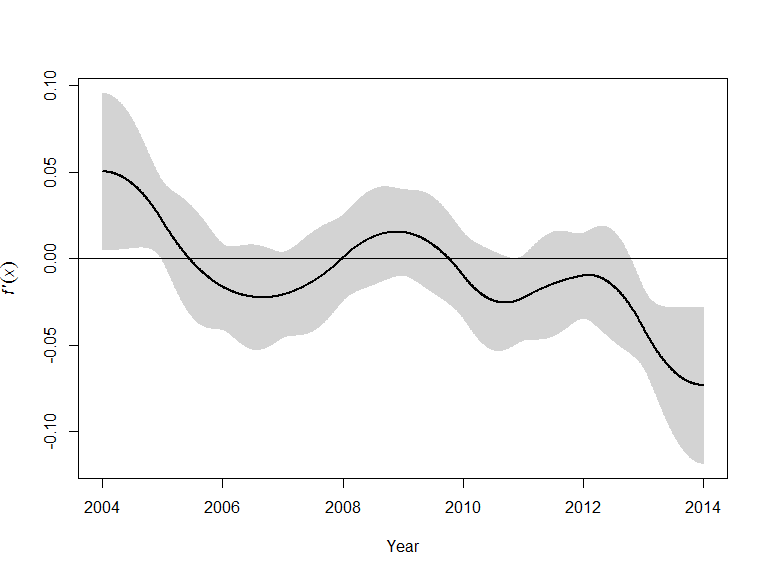
\includegraphics{BiometriaiKonf2017_FerenciKolossvary_files/figure-beamer/splinederivcivel-1.pdf}

\end{frame}

\begin{frame}[fragile]{És a nagyfinálé}

\begin{Shaded}
\begin{Highlighting}[]
\NormalTok{fit.d.CI <-}\StringTok{ }\KeywordTok{confint}\NormalTok{( fit.d, }\StringTok{"Year"} \NormalTok{)}
\NormalTok{fit.d.signif <-}\StringTok{ }\KeywordTok{signifD}\NormalTok{( pred$fit, fit.d$Year$deriv, fit.d.CI$Year$upper, fit.d.CI$Year$lower )}
\KeywordTok{xYplot}\NormalTok{( }\KeywordTok{Cbind}\NormalTok{( fit, lwr, upr )~predtime, }\DataTypeTok{data =} \NormalTok{pred, }\DataTypeTok{method =} \StringTok{"filled bands"}\NormalTok{, }\DataTypeTok{type =} \StringTok{"l"}\NormalTok{,}
        \DataTypeTok{col.fill =} \KeywordTok{gray}\NormalTok{( }\KeywordTok{seq}\NormalTok{( .}\DecValTok{825}\NormalTok{, .}\DecValTok{55}\NormalTok{, }\DataTypeTok{length =} \DecValTok{5} \NormalTok{) ), }\DataTypeTok{xlab =} \StringTok{"Year"}\NormalTok{, }\DataTypeTok{ylab =} \StringTok{""}\NormalTok{,}
        \DataTypeTok{scales =} \KeywordTok{list}\NormalTok{( }\DataTypeTok{x =} \KeywordTok{list}\NormalTok{( }\DataTypeTok{at =} \NormalTok{predtime[}\DecValTok{1}\NormalTok{]:}\KeywordTok{tail}\NormalTok{( predtime, }\DecValTok{1} \NormalTok{) ) ), }\DataTypeTok{ylim =} \KeywordTok{c}\NormalTok{( }\DecValTok{18}\NormalTok{, }\DecValTok{25} \NormalTok{) ) +}
\StringTok{  }\KeywordTok{as.layer}\NormalTok{( }\KeywordTok{xyplot}\NormalTok{( fit.d.signif$incr~predtime, }\DataTypeTok{type =} \StringTok{"l"}\NormalTok{, }\DataTypeTok{lwd =} \DecValTok{3}\NormalTok{, }\DataTypeTok{col =} \StringTok{"blue"} \NormalTok{) ) +}
\StringTok{  }\KeywordTok{as.layer}\NormalTok{( }\KeywordTok{xyplot}\NormalTok{( fit.d.signif$decr~predtime, }\DataTypeTok{type =} \StringTok{"l"}\NormalTok{, }\DataTypeTok{lwd =} \DecValTok{3}\NormalTok{, }\DataTypeTok{col =} \StringTok{"red"} \NormalTok{) )}
\end{Highlighting}
\end{Shaded}

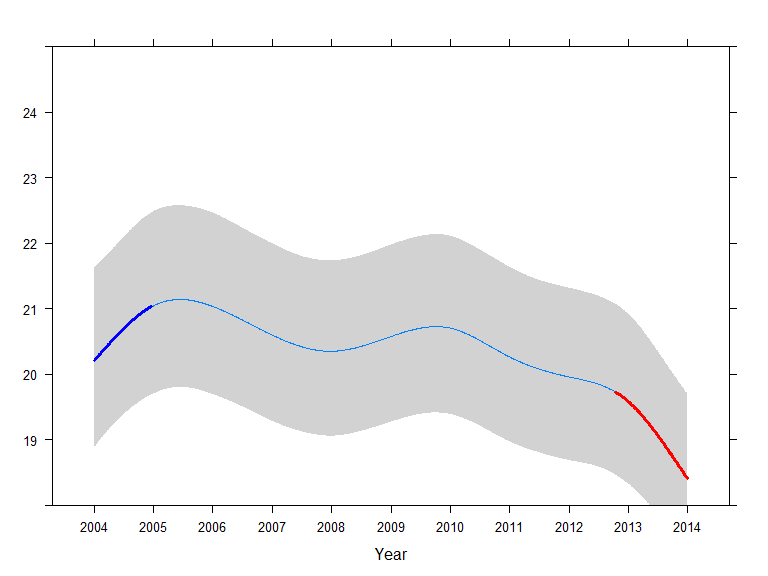
\includegraphics{BiometriaiKonf2017_FerenciKolossvary_files/figure-beamer/vegerdmeny-1.pdf}

\end{frame}

\begin{frame}{Összefoglalva}

\begin{itemize}
\tightlist
\item
  A paraméteres modellek jól interpretálhatóak, extrapolálhatóak, de
  kérdéses lehet az illeszkedésük a valósághoz
\item
  A nemparaméteres modelleknél lényegében fordított az előny/hátrány
  helyzet
\item
  A spline-okat használó (félparaméteres) modellek jó kompromisszumot
  jelentenek
\item
  A bemutatott módszerrel pedig némileg még az interpretálhatóságuk is
  javítható
\end{itemize}

\end{frame}

\end{document}
